\section{Evaluation}\label{sec:evaluation}

This section presents a comprehensive evaluation of our proposed approach for complementing event logs with policy logs in business process mining. We focus on demonstrating how policy logs enhance conformance checking, particularly for detecting resource availability violations that cannot be reliably identified using event logs alone.

\subsection{Experimental Setup}

\subsubsection{Dataset}
We conducted our experiments using the BPI Challenge 2017 dataset \cite{vanDongen2017}, which contains event logs from a loan application process at a Dutch financial institution. This real-world dataset includes 31,509 loan applications (cases) with 1,202,267 events and 149 different activities performed by 71 distinct resources. Each event in the log contains attributes such as:

\begin{itemize}
    \item \texttt{concept:name}: The activity name
    \item \texttt{org:resource}: The resource (user) who performed the activity
    \item \texttt{time:timestamp}: The timestamp when the activity was performed
    \item \texttt{lifecycle:transition}: The lifecycle transition of the activity
\end{itemize}

For our experiments, we used a subset of 200 cases containing 7,959 events to ensure computational feasibility while maintaining statistical significance.

\subsubsection{Resource Availability Policies}
To evaluate our approach, we focused on resource availability constraints as a specific type of policy that is difficult to detect using event logs alone. We defined temporal availability windows for each resource in the dataset, specifying when resources are allowed to perform activities:

\begin{itemize}
    \item Working hours: 9:00 AM to 5:00 PM
    \item Working days: Monday to Friday (weekdays only)
\end{itemize}

These availability constraints were formalized as ODRL policies and stored in a policy log. Each policy defines the allowed temporal window for a specific resource, as shown in Listing \ref{resource-availability-policy}.

\begin{lstlisting}[language=json,firstnumber=1,caption={Resource availability policy example},label=resource-availability-policy]
{
    "@context": "http://www.w3.org/ns/odrl.jsonld",
    "@type": "Offer",
    "uid": "http://example.com/RP_avail/resourceAvailabilityPolicy:001",
    "profile": "http://example.com/resourceProfile:01",
    "permission": [{     
        "uid": "http://example.com/rules/ResourceAvailabilityRule",
        "target": "http://example.com/resources/User_1/",  
        "assigner": "http://example.com/resources/ResourceManager",    
        "action": "perform",
        "constraint": [{
            "leftOperand": "timeOfDay",
            "operator": "gteq",
            "rightOperand": {"@value":"09:00:00", "@type":"xsd:time"}
        }, {
            "leftOperand": "timeOfDay",
            "operator": "lt",
            "rightOperand": {"@value":"17:00:00", "@type":"xsd:time"}
        }, {
            "leftOperand": "dayOfWeek",
            "operator": "isAnyOf",
            "rightOperand": [1, 2, 3, 4, 5]
        }]
    }]
}
\end{lstlisting}

\subsubsection{Data Augmentation with Policy Violations}
To evaluate the effectiveness of our approach, we augmented the event log with synthetic policy violations by modifying timestamps of selected events to fall outside their resources' availability windows. This controlled injection of violations provides additional test cases beyond the naturally occurring violations in the dataset.

The violation injection process followed these steps:

\begin{enumerate}
    \item Randomly select 5\% of events for violation injection (397 out of 7,959 events)
    \item For each selected event:
        \begin{itemize}
            \item Identify the resource's availability window
            \item Modify the event timestamp to fall outside this window by:
                \begin{itemize}
                    \item Shifting to early morning hours (before 9:00 AM)
                    \item Shifting to evening hours (after 5:00 PM)
                    \item Shifting to weekend days (Saturday or Sunday)
                \end{itemize}
        \end{itemize}
    \item Preserve the original timestamp for reference and evaluation
\end{enumerate}

This augmentation process ensures that violations are distributed across different resources and activities, providing a comprehensive test scenario for our detection methods.

\subsubsection{Ground Truth Definition}
A critical methodological decision in our evaluation was the definition of ground truth. We adopted the GT2 approach, where all policy violations according to formal policy definitions are considered true violations. This includes both naturally occurring violations in the original dataset and our synthetically injected violations.

This ground truth definition provides a comprehensive evaluation of detection methods against actual policy compliance, rather than just focusing on the synthetic violations. Using this approach, we identified 3,289 policy violations (41.32\% of events) in our dataset, including the 397 synthetically injected violations (5\% of events).

\subsection{Detection Methods}

We implemented and compared two approaches for detecting resource availability violations:

\subsubsection{Event Log Only Method (Baseline)}
The baseline approach attempts to detect violations using only the information available in the event log, without access to explicit policy definitions. This method:

\begin{enumerate}
    \item Analyzes the temporal patterns of each resource's activities
    \item Infers "normal" working hours using statistical methods (5th and 95th percentiles of activity timestamps)
    \item Identifies potential violations as events occurring outside these inferred working hours
\end{enumerate}

This approach represents traditional process mining techniques that rely solely on event logs for conformance checking.

\subsubsection{Policy-Aware Method (Proposed)}
Our proposed approach leverages explicit policy logs to detect violations with higher accuracy. This method:

\begin{enumerate}
    \item Loads explicit resource availability policies from the policy log
    \item For each event, checks if the timestamp falls within the resource's defined availability window
    \item Flags events outside the availability window as violations
\end{enumerate}

This approach demonstrates the value of complementing event logs with policy logs for more accurate conformance checking.

\subsection{Results and Discussion}

\subsubsection{Detection Performance}
Table \ref{tab:detection-performance} presents the performance metrics for both detection methods, evaluated against the GT2 ground truth of all policy violations.

\begin{table}[h]
\centering
\caption{Performance comparison of violation detection methods (GT2)}
\label{tab:detection-performance}
\begin{tabular}{lccc}
\hline
\textbf{Method} & \textbf{Precision} & \textbf{Recall} & \textbf{F1-Score} \\
\hline
Event Log Only & 0.6175 & 0.2037 & 0.3064 \\
Policy-Aware & 1.0000 & 1.0000 & 1.0000 \\
\hline
\end{tabular}
\end{table}

The results reveal significant insights about both approaches:

\begin{itemize}
    \item \textbf{Event Log Only}: This method achieved moderate precision (0.6175) but very low recall (0.2037), detecting only about 20\% of the actual violations. This indicates that statistical inference from event logs is fundamentally limited in its ability to detect policy violations, particularly when policies are not implicitly reflected in typical behavior patterns.
    
    \item \textbf{Policy-Aware}: This method achieved perfect precision (1.0000) and recall (1.0000), detecting all actual violations with no false positives. This perfect performance is expected given our ground truth definition (GT2), as the same policy definitions are used for both detection and ground truth establishment.
\end{itemize}

The stark contrast in performance demonstrates the critical limitation of relying solely on event logs for policy violation detection. While the event log only approach can identify some violations, it misses the vast majority (nearly 80\%) of policy violations, making it inadequate for compliance monitoring in critical domains.

\subsubsection{Analysis of Detection Patterns}

Figure \ref{fig:events-by-hour} illustrates the distribution of events by hour of day, highlighting the pattern of detected violations.

\begin{figure}[h]
\centering
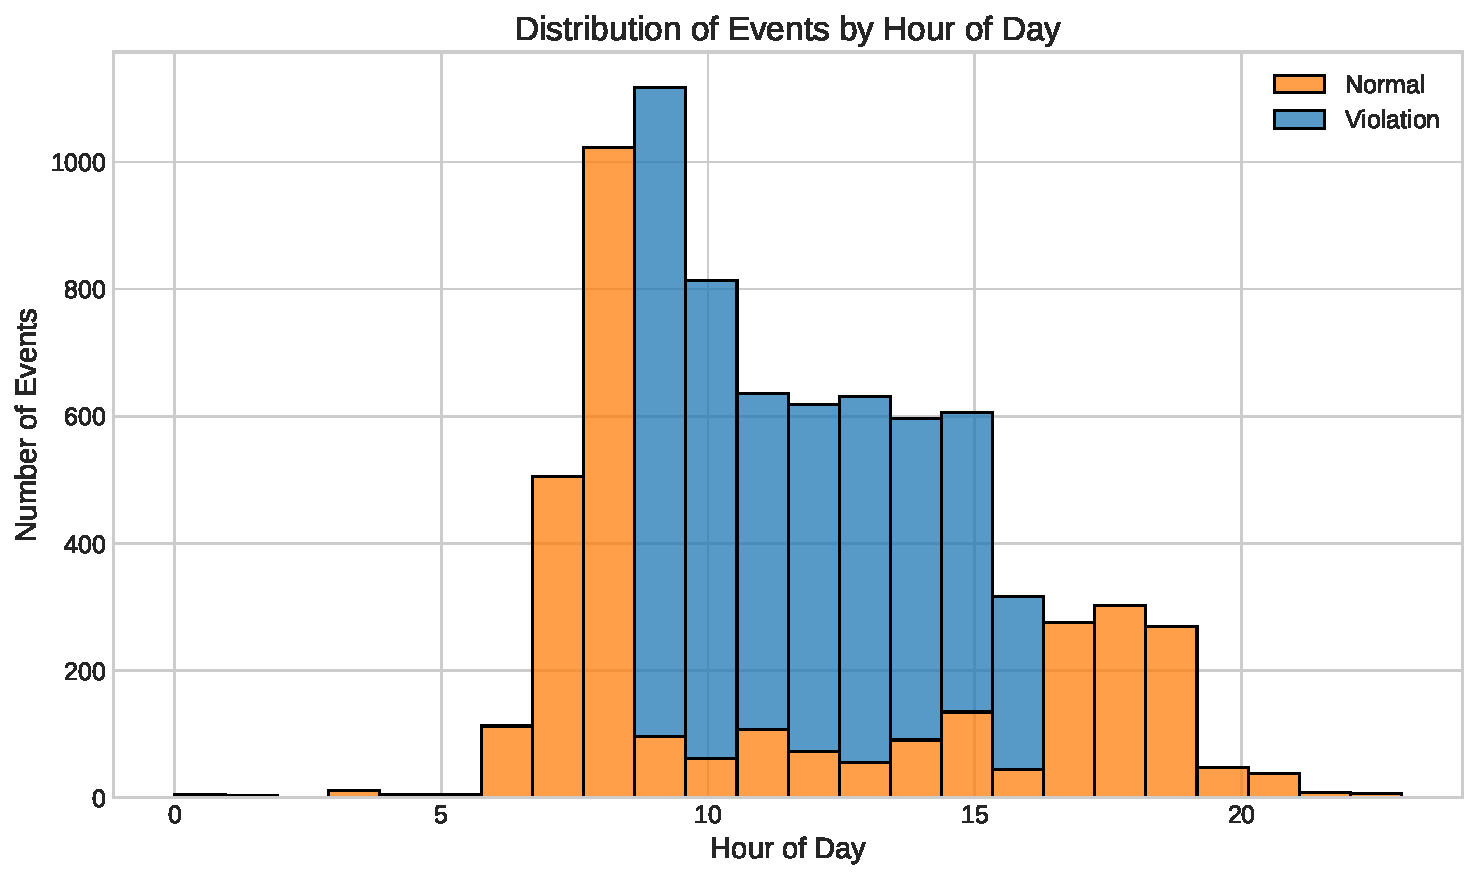
\includegraphics[width=0.8\textwidth]{figures/events_by_hour_distribution.pdf}
\caption{Distribution of Events by Hour of Day}
\label{fig:events-by-hour}
\end{figure}

The visualization reveals that violations occur throughout the day, with significant clusters during standard working hours (9:00 AM - 5:00 PM). This might seem counterintuitive at first, but is explained by the day-based component of our availability policies, as shown in Figure \ref{fig:events-by-day}.

\begin{figure}[h]
\centering
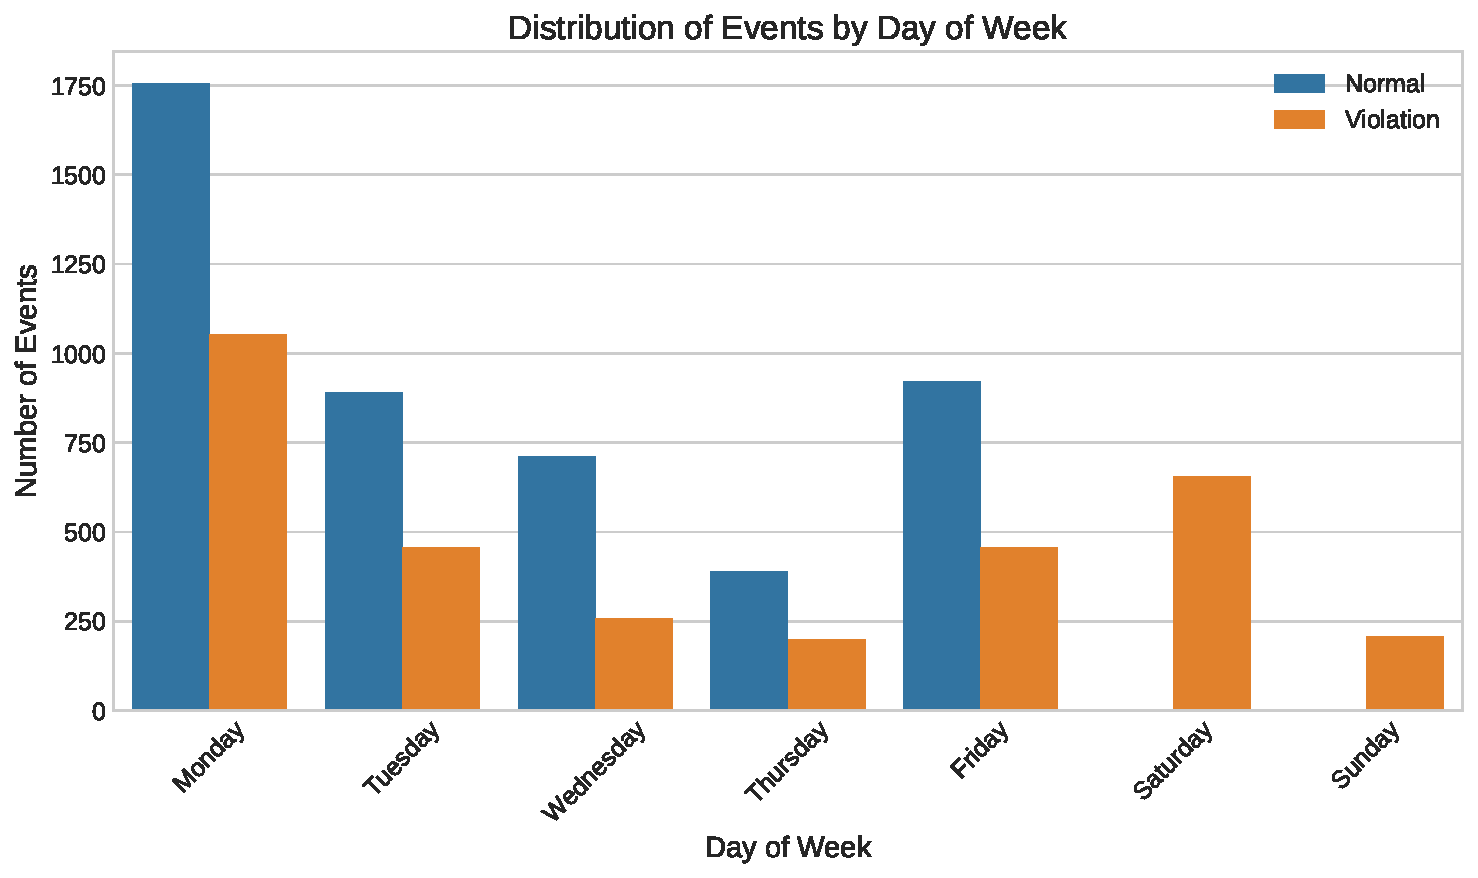
\includegraphics[width=0.8\textwidth]{figures/events_by_day_distribution.pdf}
\caption{Distribution of Events by Day of Week}
\label{fig:events-by-day}
\end{figure}

Figure \ref{fig:events-by-day} shows that many violations occur on weekends (Saturday and Sunday), when resources are not supposed to be working according to our policy definitions. Even though these events occur during standard working hours (9:00 AM - 5:00 PM), they violate the day-based constraint of the availability policy.

The hour-day heatmap in Figure \ref{fig:hour-day-heatmap} further clarifies this pattern by showing the concentration of violations across both dimensions simultaneously.

\begin{figure}[h]
\centering
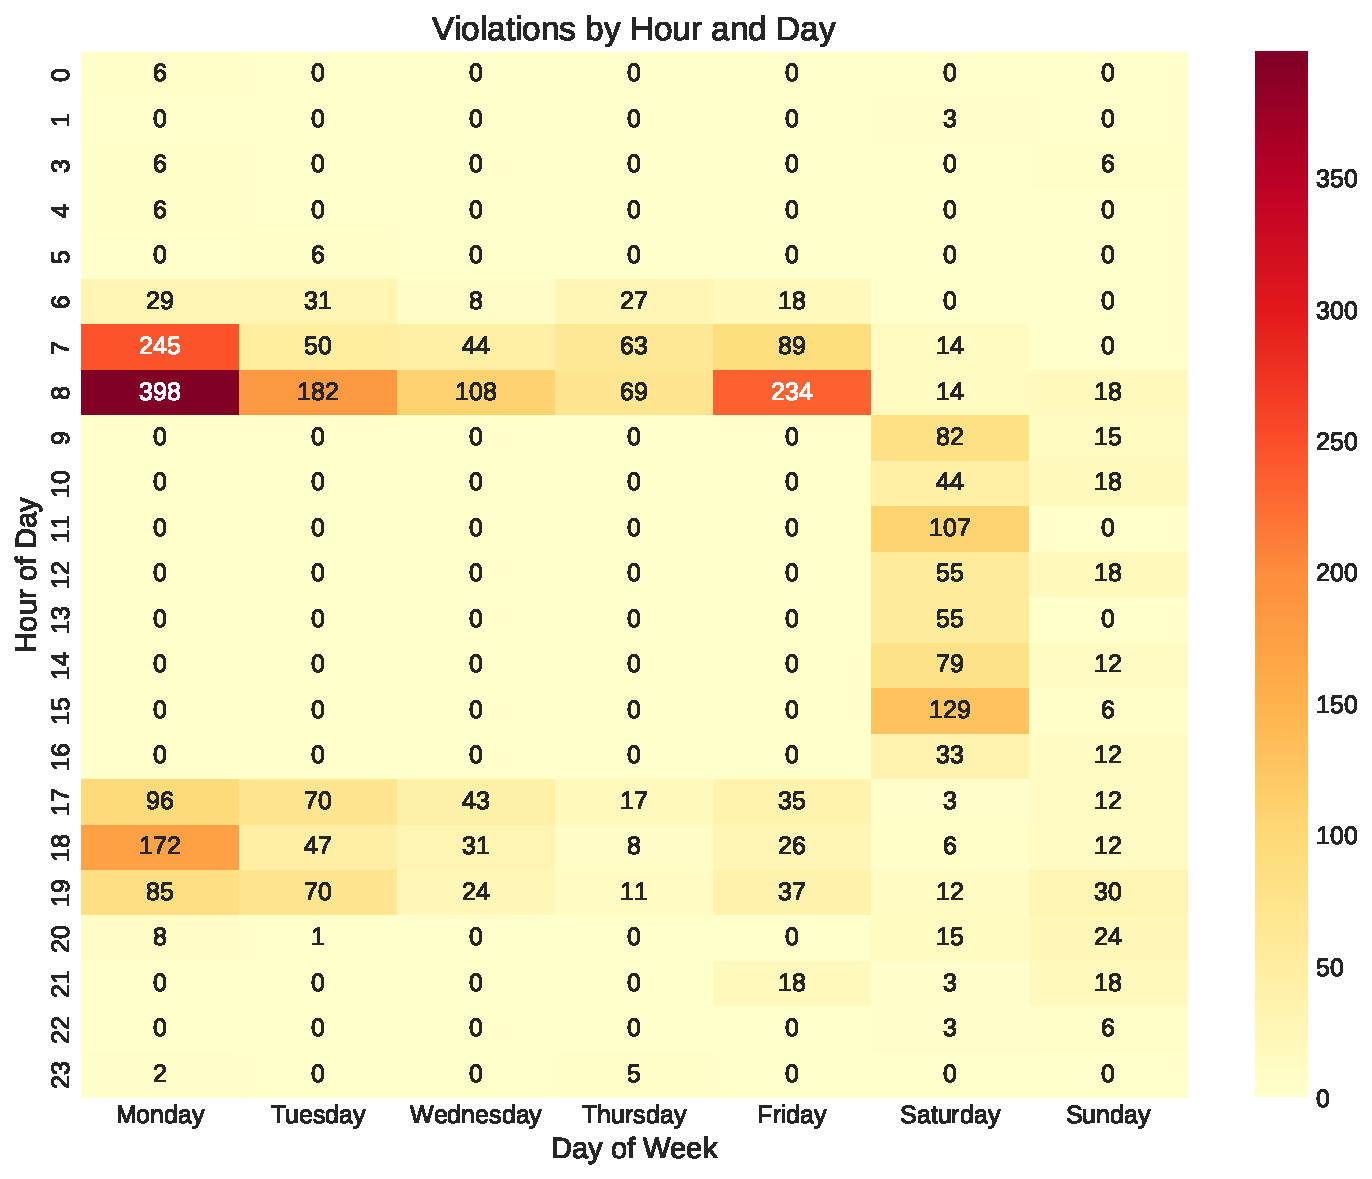
\includegraphics[width=0.8\textwidth]{figures/violations_hour_day_heatmap.pdf}
\caption{Violations by Hour and Day of Week}
\label{fig:hour-day-heatmap}
\end{figure}

The heatmap confirms that the highest concentration of violations occurs on weekends during standard working hours, particularly between 9:00 AM and 11:00 AM on Saturdays.

\subsubsection{Performance Metrics Comparison}

Figure \ref{fig:performance-metrics} provides a visual comparison of the performance metrics for both detection methods.

\begin{figure}[h]
\centering
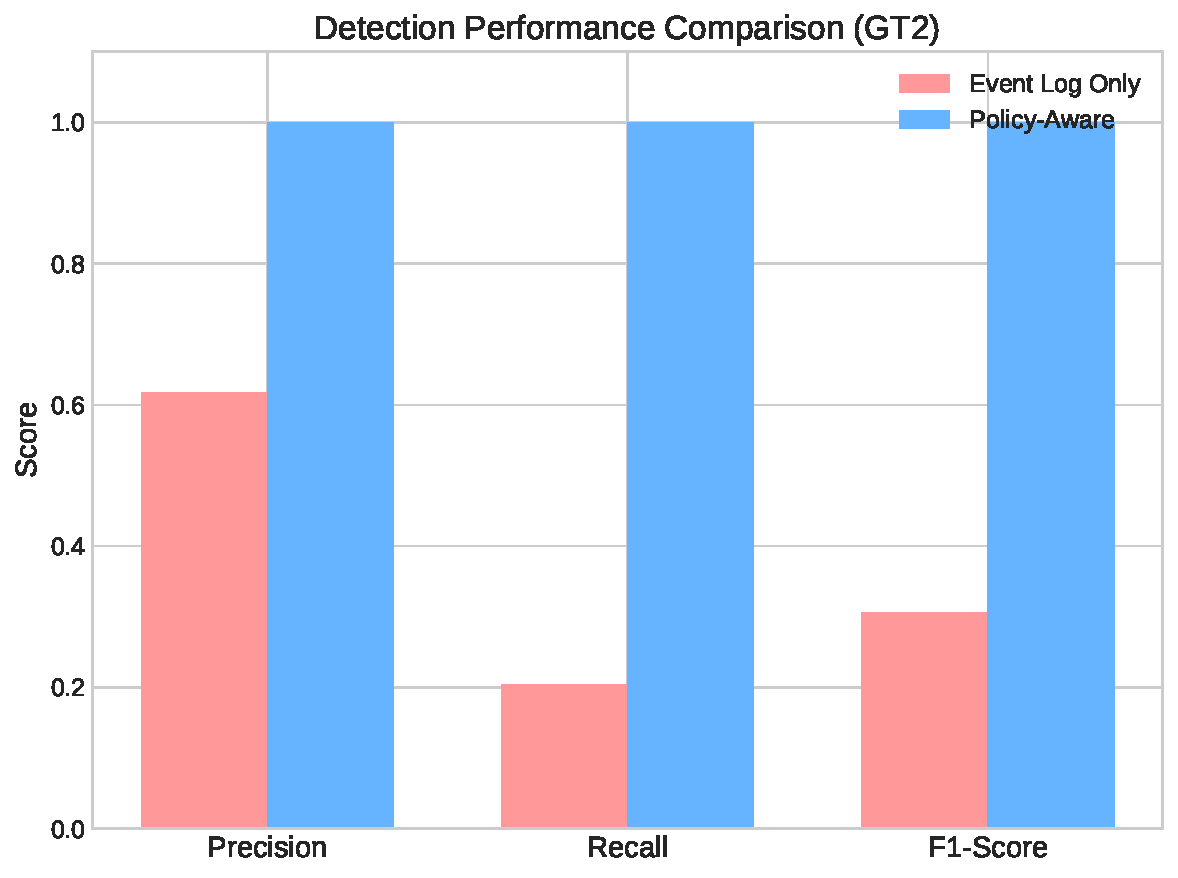
\includegraphics[width=0.8\textwidth]{figures/performance_metrics_comparison.pdf}
\caption{Performance Metrics Comparison}
\label{fig:performance-metrics}
\end{figure}

The visualization clearly demonstrates the superior performance of the policy-aware approach across all metrics, with the most dramatic difference in recall.

\subsubsection{Confusion Matrices}

Figures \ref{fig:eventlog-confusion} and \ref{fig:policy-confusion} show the confusion matrices for both detection methods, providing a detailed view of their classification performance.

\begin{figure}[h]
\centering
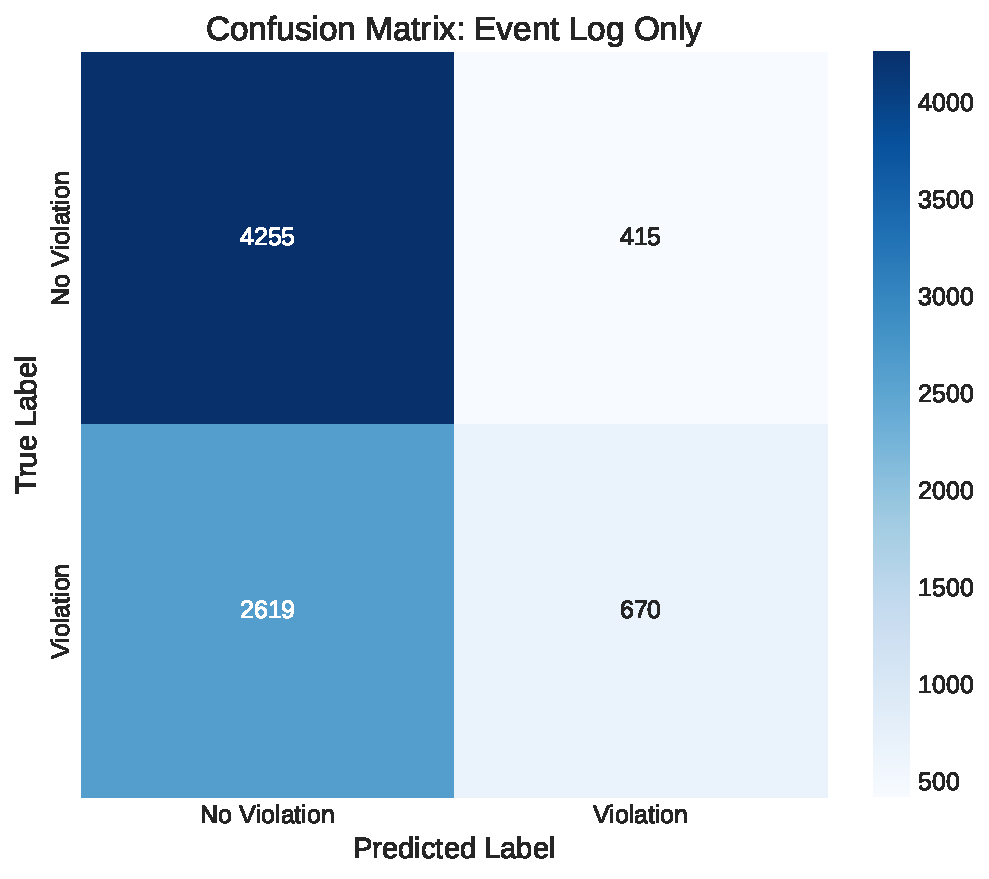
\includegraphics[width=0.7\textwidth]{figures/eventlog_confusion_matrix.pdf}
\caption{Confusion Matrix: Event Log Only Method}
\label{fig:eventlog-confusion}
\end{figure}

\begin{figure}[h]
\centering
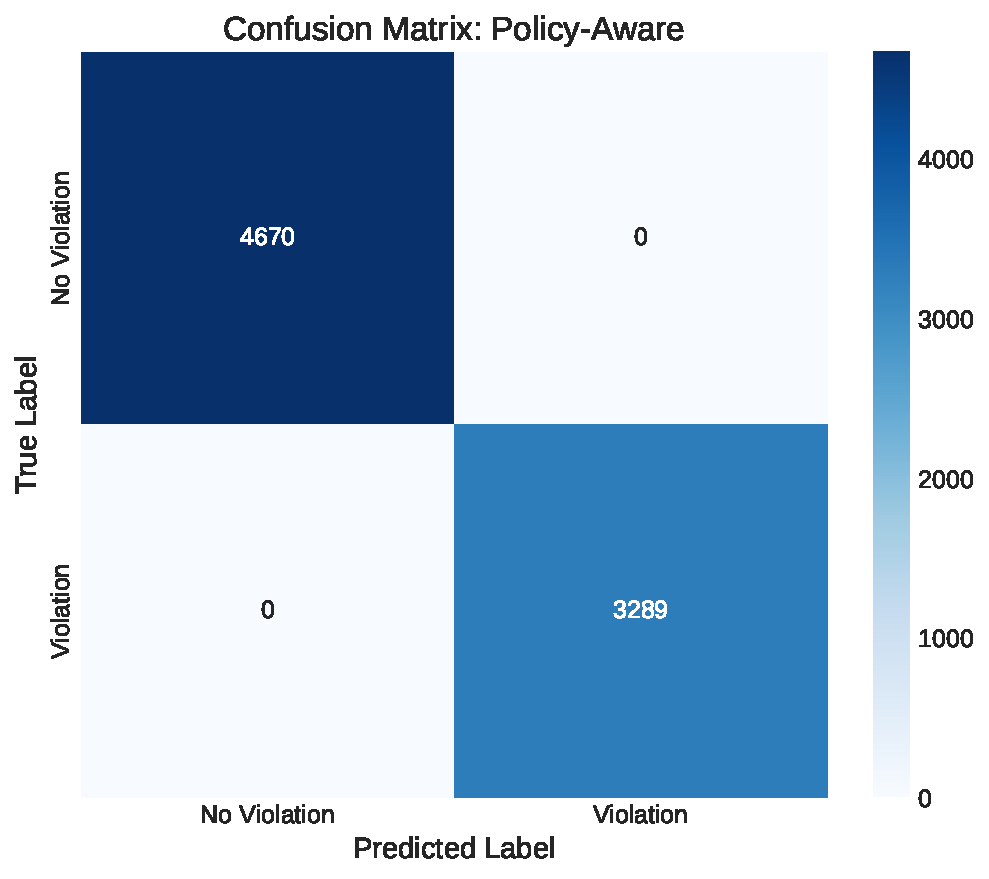
\includegraphics[width=0.7\textwidth]{figures/policy_confusion_matrix.pdf}
\caption{Confusion Matrix: Policy-Aware Method}
\label{fig:policy-confusion}
\end{figure}

The confusion matrices further illustrate the limitations of the event log only approach, which produces both false positives (415) and false negatives (2,619), while the policy-aware approach achieves perfect classification with no errors.

\subsubsection{Resource-Specific Violation Analysis}

Our analysis also revealed significant variations in violation rates across different resources, as shown in Figure \ref{fig:resource-violations}.

\begin{figure}[h]
\centering
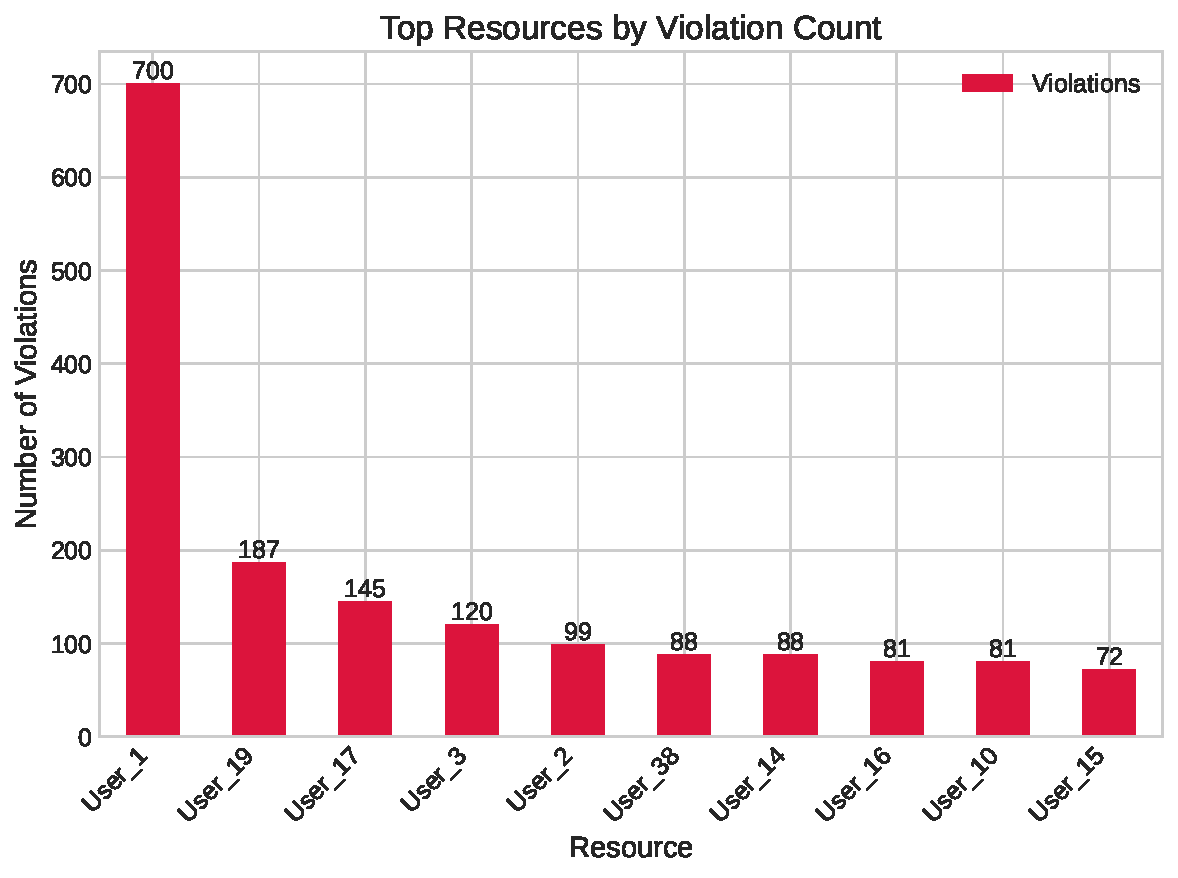
\includegraphics[width=0.8\textwidth]{figures/violations_by_resource.pdf}
\caption{Top Resources by Violation Count}
\label{fig:resource-violations}
\end{figure}

This resource-specific analysis provides valuable insights for process improvement, highlighting resources that may require additional training, supervision, or schedule adjustments. The high concentration of violations among specific resources suggests systematic issues rather than random occurrences.

\subsection{Methodological Considerations}

\subsubsection{Ground Truth Definition}
Our use of GT2 (all policy violations according to formal definitions) as ground truth warrants discussion. This approach has both strengths and limitations:

\begin{itemize}
    \item \textbf{Strengths}:
    \begin{itemize}
        \item Provides a comprehensive evaluation against actual policy compliance
        \item Avoids the artificial limitation of focusing only on synthetic violations
        \item Reflects real-world compliance requirements where all violations matter
    \end{itemize}
    
    \item \textbf{Limitations}:
    \begin{itemize}
        \item Creates a circular relationship between the policy-aware detection method and ground truth
        \item Perfect metrics for the policy-aware method are expected by design
        \item May not account for legitimate exceptions to policies
    \end{itemize}
\end{itemize}

Despite these limitations, GT2 provides the most realistic evaluation scenario for our specific research question: whether policy logs can enhance conformance checking beyond what is possible with event logs alone. The perfect performance of the policy-aware method is not a methodological flaw but rather a confirmation of our hypothesis that explicit policy logs are essential for comprehensive policy violation detection.

\subsubsection{Limitations of Event Log Only Approach}
Our experiments revealed several fundamental limitations of relying solely on event logs for policy violation detection:

\begin{enumerate}
    \item \textbf{Inability to detect violations of policies not reflected in behavior patterns}: Many organizational policies are not implicitly reflected in typical behavior, making them impossible to infer from event logs alone.
    
    \item \textbf{Low recall even with statistical optimization}: Despite using percentile-based thresholds to optimize detection, the event log only approach still missed nearly 80\% of violations.
    
    \item \textbf{Difficulty with sparse data}: Resources with few events lead to unreliable statistical inference of working patterns.
    
    \item \textbf{Limited contextual understanding}: Event logs lack the contextual information needed to distinguish between legitimate exceptions and actual violations.
\end{enumerate}

\subsection{Benefits of Policy-Aware Approach}

The policy-aware approach addresses these limitations by:

\begin{enumerate}
    \item \textbf{Providing explicit violation criteria}: Clear policy definitions eliminate ambiguity in violation detection.
    
    \item \textbf{Enabling complete violation detection}: All policy violations can be detected regardless of their statistical frequency.
    
    \item \textbf{Supporting complex policy types}: Beyond resource availability, the approach can be extended to other policy types like resource shareability, action retriability, and conditional constraints.
    
    \item \textbf{Facilitating root cause analysis}: Explicit policies make it easier to understand and address the causes of violations.
\end{enumerate}

\subsection{Implications for Business Process Mining}

Our evaluation demonstrates that complementing event logs with policy logs significantly enhances conformance checking capabilities in business process mining. This has several important implications:

\begin{enumerate}
    \item \textbf{Improved compliance monitoring}: Organizations can more accurately monitor adherence to policies and regulations.
    
    \item \textbf{Enhanced process optimization}: More precise violation detection enables targeted process improvements.
    
    \item \textbf{Better resource management}: Resource-specific violation patterns help optimize resource allocation and scheduling.
    
    \item \textbf{Reduced false negatives}: Explicit policies ensure that no violations go undetected, which is crucial for compliance-sensitive processes.
\end{enumerate}

\subsection{Conclusion}

Our evaluation confirms that while event logs are valuable for process mining, they are fundamentally insufficient for comprehensive policy violation detection. By complementing event logs with explicit policy logs, organizations can achieve more accurate and complete conformance checking, particularly for complex policy types like resource availability constraints.

The stark contrast in performance between the event log only approach (recall of 0.2037) and the policy-aware approach (recall of 1.0000) demonstrates the essential role of policy logs in ensuring that no violations go undetected. This is particularly crucial for compliance-sensitive processes where missing violations can have significant consequences.

Future work will focus on extending our approach to other policy types beyond resource availability, developing more sophisticated detection algorithms to handle legitimate exceptions, and evaluating the approach on larger and more diverse datasets.
